\documentclass[a4paper, 12pt]{article}
\usepackage[T1]{fontenc}
\usepackage{lmodern}
\usepackage{color}
\usepackage{amsfonts}
\usepackage{epstopdf}
\usepackage{matlab}
%\documentclass{book}
\usepackage{blindtext}
\usepackage{hyperref}
\usepackage[brazil]{babel}
\usepackage{amssymb}
\usepackage[utf8]{inputenc}
\usepackage{amsmath}
\usepackage{indentfirst}
\usepackage{graphicx}
\usepackage{multicol,lipsum}
\usepackage[a4paper,
top=3cm, left=3cm, bottom=3cm, right=3cm]{geometry}
\usepackage{setspace}
\usepackage{multirow}
\usepackage{float}
\usepackage[dvipsnames]{xcolor}
\usepackage[table]{xcolor}
%\usepackage{pdflscape}
\usepackage[DIV=15]{typearea}
\usepackage[nottoc]{tocbibind}
\usepackage[sort,numbers]{natbib}
%\usepackage{cite}
\usepackage{matlab}

\usepackage[utf8]{inputenc}
\usepackage[T1]{fontenc}
\usepackage{lmodern}
\usepackage{graphicx}
\usepackage{color}
\usepackage{hyperref}
\usepackage{amsmath}
\usepackage{amsfonts}
\usepackage{epstopdf}
\usepackage[table]{xcolor}
\usepackage{matlab}


\documentclass[letterpaper]{article}
% bib pack %%%%%%%%%%%%%%%%%%%%%%%%%%%%%%%%%%%%%%%%%%%%%%%%%%%%%%%%%%%%%%%%%%%%%
\usepackage[utf8]{inputenc}
\usepackage{geometry}
    \geometry{left=3cm,right=2cm,top=2cm,bottom=2cm}
%
\usepackage[spanish]{babel}
%
\usepackage[fixlanguage]{babelbib}
    \bibliographystyle{babunsrt}
%
\usepackage{url}

\begin{document}
%\maketitle

\begin{titlepage}
	\begin{center}
		

\vspace{10pt}
%\begin{figure}[H][!ht]
%\centering
%
\includegraphics{puc-rio-logo.png}

%\end{figure}
\begin{figure}[!ht]
\centering

\includegraphics{images/puc-rio-logo.png}
\end{figure}
\huge{Dinâmica de Sistemas}
        \vspace{70pt}
        
		\textbf{ENG1730}
		\textbf{\large{\\ }}
		
		\vspace{30pt}
		\textbf{\small{\\Lista 03}}
		\vspace{75pt}
		
	\end{center}
	
	\begin{flushleft}
		\begin{tabbing}
			Aluno(a)\qquad\qquad\=\>Paloma Fernanda Loureiro Sette - 1621595\\
			
			Professor(a)\>João Carlos Virgolino Soares\\
	\end{tabbing}
		  
	\end{flushleft}
	\begin{center}
		%\vspace{\fill}
		\vspace{215pt}
		Rio de Janeiro, 15 de Setembro de 2022
	\end{center}
\end{titlepage}
%%%%%%%%%%%%%%%%%%%%%%%%%%%%%%%%%%%%%%%%%%%%%%%%%%%%%%%%%%%
\newpage
\tableofcontents
\thispagestyle{empty}

\newpage
\pagenumbering{arabic}

\newpage

%\newcommand{\listequationsname}{Lista de Equações}
%\newlistof{myequations}{equ}{\listequationsname}
%\newcommand{\myequations}[1]{%
%\addcontentsline{equ}{myequations}{\protect\numberline{\theequation}#1}\par}

%\listofmyequations
\newpage


\newpage

\listoffigures
\thispagestyle{empty}

\newpage
%%%%%%%%%%%%%%%%%%%%%%%%%%%%%%%%%%%%%%%%%%%%%%%%%%%%%%%%%
%%%%%%%%%%%%%%%%%%%%%%%%%%%%%%%%%%%%%%%%%%%%%%%%%%%

\newpage

\thispagestyle{empty}

\newpage

\section{Introdução}
Este relatório refere-se ao terceiro trabalho da disciplina de Dinâmica de Sistemas, ENG1730, de 2022.2. Trataremos da modelagem matemática de sistemas rotacionais polia-mola e polia-massa-mola.

\section{Questão 01}
A figura a seguir mostra um disco homogêneo de raio $R$ e massa $m$ preso pelo teto que pode girar em torno do seu centro de massa. O disco é envolvido por um fio conectado a duas molas pré-deformadas. Cada mola é pré-deformada com um valor $x$. Assumindo que o disco está rotacionado inicialmente por um ângulo pequeno $\theta$ e depois é solto, obtenha o modelo matemático do sistema.

\begin{figure}[H]
\centering
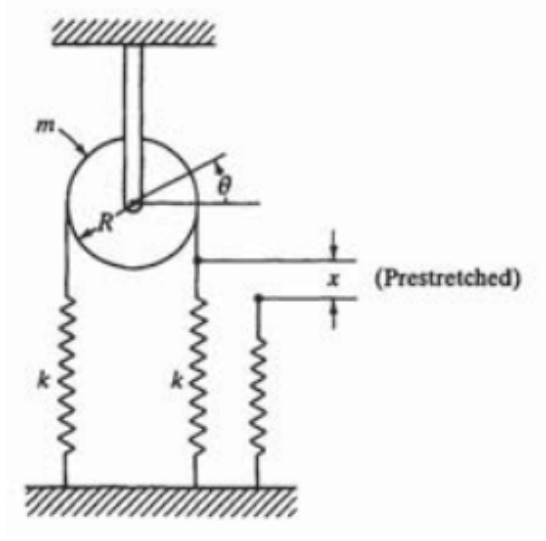
\includegraphics[scale = 0.6]{images/sistema.png}
\label{filtro1}
\caption{Sistema - questão 01}
\end{figure}

\subsection{Modelo matemático do sistema}
Se o disco for girado em um ângulo $\theta$, então sabemos que a mola da direita será esticada a uma deformação $x + R\theta$ e a mola da esquerda, consequentemente, sofrerá uma deformação de $x - R\theta$. Portanto, teremos,

\begin{equation}\label{eq}
    J\ddot \theta =  k(x - R\theta)R - k(x+R\theta)R
\end{equation}\\

Onde sabemos que o momento de inércia $J$ é 

\begin{equation}
    J = \frac{1}{2} mR^2    
\end{equation}

Então, se simplificarmos a equação \ref{eq}, obteremos o modelo matemático do sistema:

\begin{equation}
    \ddot \theta = - \frac{4k}{m} \theta
\end{equation}



\newpage
\section{Questão 02}

A figura a seguir mostra um sistema massa-mola-polia. O momento de inércia da polia em relação ao seu eixo de rotação é $J$ e o seu raio é $R$. Assuma que o sistema está inicialmente em equilíbrio. O peso da massa $m$ causa uma deflexão estática na mola tal que $k\delta = mg$ . Assumindo que o deslocamento da massa $x$ é medido a partir da posição de equilíbrio, obtenha o modelo matemático do sistema.

\begin{figure}[H]
\centering
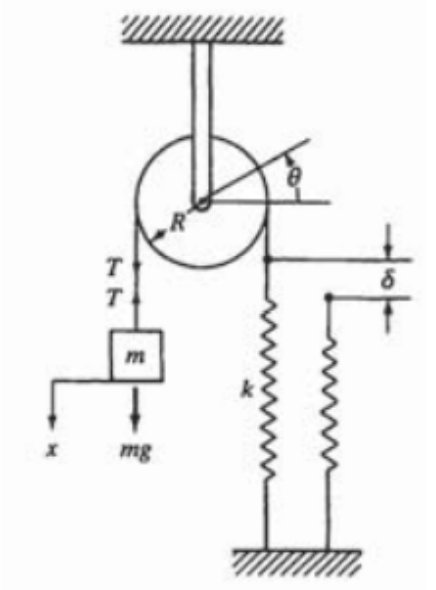
\includegraphics[scale = 0.6]{images/sistema2.png}
\label{filtro1}
\caption{Sistema massa-mola - questão 01}
\end{figure}

\subsection{Modelo matemático do sistema}

Considerando a Segunda Lei de Newton, sabemos que

\begin{equation}]\label{eq2}
    m \ddot x = -T
\end{equation}

Sendo $T$ a tensão aplicada ao fio pela massa $m$. Para o movimento rotacional da polia, teremos

\begin{equation}\label{eq3}
    J \ddot\theta = TR - kxR
\end{equation}

Neste caso, podemos substituir a tensão $T$ por $m\ddot x$, i.e. \ref{eq2} $\xrightarrow[]{}$ \ref{eq3}.\\

\begin{equation}\label{eq3}
    J \ddot \theta = -m \ddot x R - kxR
\end{equation}

Como sabemos também que $x = R\theta$, poderemos substituir em \ref{eq3}. Assim, teremos:

\begin{equation}
    J \ddot \theta = -m \ddot \theta R^2 - kR^2\theta
\end{equation}

\begin{equation}
    \ddot \theta ( J + m R^2) + kR^2\theta = 0
\end{equation}\\

Logo, obtemos o modelo matemático:

\begin{equation}
    \ddot \theta = - \frac{kR^2}{J + m R^2} \theta
\end{equation}





\end{document}